\chapter{Full \texorpdfstring{$\delta_{0}$}{delta\_0} family sweep (abstract sensitivity)}
\label{app:delta0-families}

This appendix expands Section~\ref{sec:delta0_oracle}. The whole
construction is an abstract sensitivity study: the operational default
of the report is the admissible scale $\delta_{0}=c\,f(\mathbf{w}_{0})$,
calibrated on principled grounds without reference to $f^{*}$
(Section~\ref{sec:dsm_parameters}). The $f^{*}$-based scale below is
reported only as a reference; it is not used to choose any parameter.

We compare Family~A $\delta_{0}=c\,f(\mathbf{w}_{0})$ against the
(inadmissible) Family~C $\delta_{0}=c\,f^{*}$ over
$c\in\{0.01,0.05,0.1,0.5,1\}$ on five instances. On four of the five
$f^{*}$ is CVXPY-verified (\texttt{CLARABEL}, cross-validated against the
IRLS-converged value to relative agreement below $10^{-9}$); on
\texttt{california}~$H=200$ the size puts CVXPY beyond a reasonable
budget and we substitute the IRLS-converged proxy --- an internal
double-circularity (the proxy comes from the algorithm being compared,
and is then fed back as $f^{*}$ to define the oracle scale) that we
flag here so the row is read as illustrative, not as a validation of the
calibration. The instance configurations are summarised in
Table~\ref{tab:delta0-families-summary}.

Family~B $\delta_{0}=c\,\tfrac12\norm{\mathbf{X}\mathbf{w}_{0}-\mathbf{y}}^{2}$
(the smooth-part-only variant of A) is plotted for completeness but is
not adopted: it has no theoretical preference over A and is empirically
comparable.

The \texttt{california}~$H=50$ and $H=200$ rows are run from the cold
start $\mathbf{w}_{0}=\mathbf{0}$ because the OLS warm start on those
instances already sits very close to $f^{*}$
(Section~\ref{sec:warm_cold}); the warm-started run would leave SGPTL
nothing to optimise and the three families would coincide at the
starting gap.

\begin{table}[H]
    \centering
    \small
    \setlength{\tabcolsep}{4pt}
    \begin{tabular}{lrrll}
        \toprule
        instance & seeds & $M\times H$ & start & $f^{*}$ source \\
        \midrule
        synthetic               & 5 & $300\times 100$  & OLS warm & CVXPY-verified \\
        \texttt{diabetes}~$H=50$  & 1 & $354\times 50$   & OLS warm & CVXPY-verified \\
        \texttt{diabetes}~$H=200$ & 1 & $354\times 200$  & OLS warm & CVXPY-verified \\
        \texttt{california}~$H=50$  & 1 & $16512\times 50$  & cold $\mathbf{w}_{0}=\mathbf{0}$ & CVXPY-verified \\
        \texttt{california}~$H=200$ & 1 & $16512\times 200$ & cold $\mathbf{w}_{0}=\mathbf{0}$ & IRLS-converged proxy \\
        \bottomrule
    \end{tabular}
    \caption{Instances used in the $\delta_{0}$ family sweep.
    \texttt{california} runs cold because the OLS solution coincides with
    $f^{*}$ to machine precision at $\lambda_\text{LASSO}=0.1$. All runs
    share $\lambda_\text{LASSO}=0.1$, $i_{\max}=8000$, $\rho=0.7$,
    $\gamma_{\min}=0.05$, $\beta=1$, $R=1$.}
    \label{tab:delta0-families-summary}
\end{table}

Across every instance, in the regime where SGPTL is optimising,
Family~A and the oracle Family~C agree within a factor of two
(Table~\ref{tab:delta0-ratio}). The single exception is
\texttt{diabetes}~$H=50$ at $c\ge 0.5$, where both scales stall at a
common plateau $\bar f^{i}-f^{*}\approx 1.4\cdot 10^{-1}$ because the
over-aggressive $\delta_{0}$ overshoots the sufficient-descent test from
the first iteration and only the travel-distance counter drives
progress; they coincide there because neither recovers from the initial
overshoot, which is a regime limit of the sweep rather than a statement
about the calibration.

\begin{figure}[H]
    \centering
    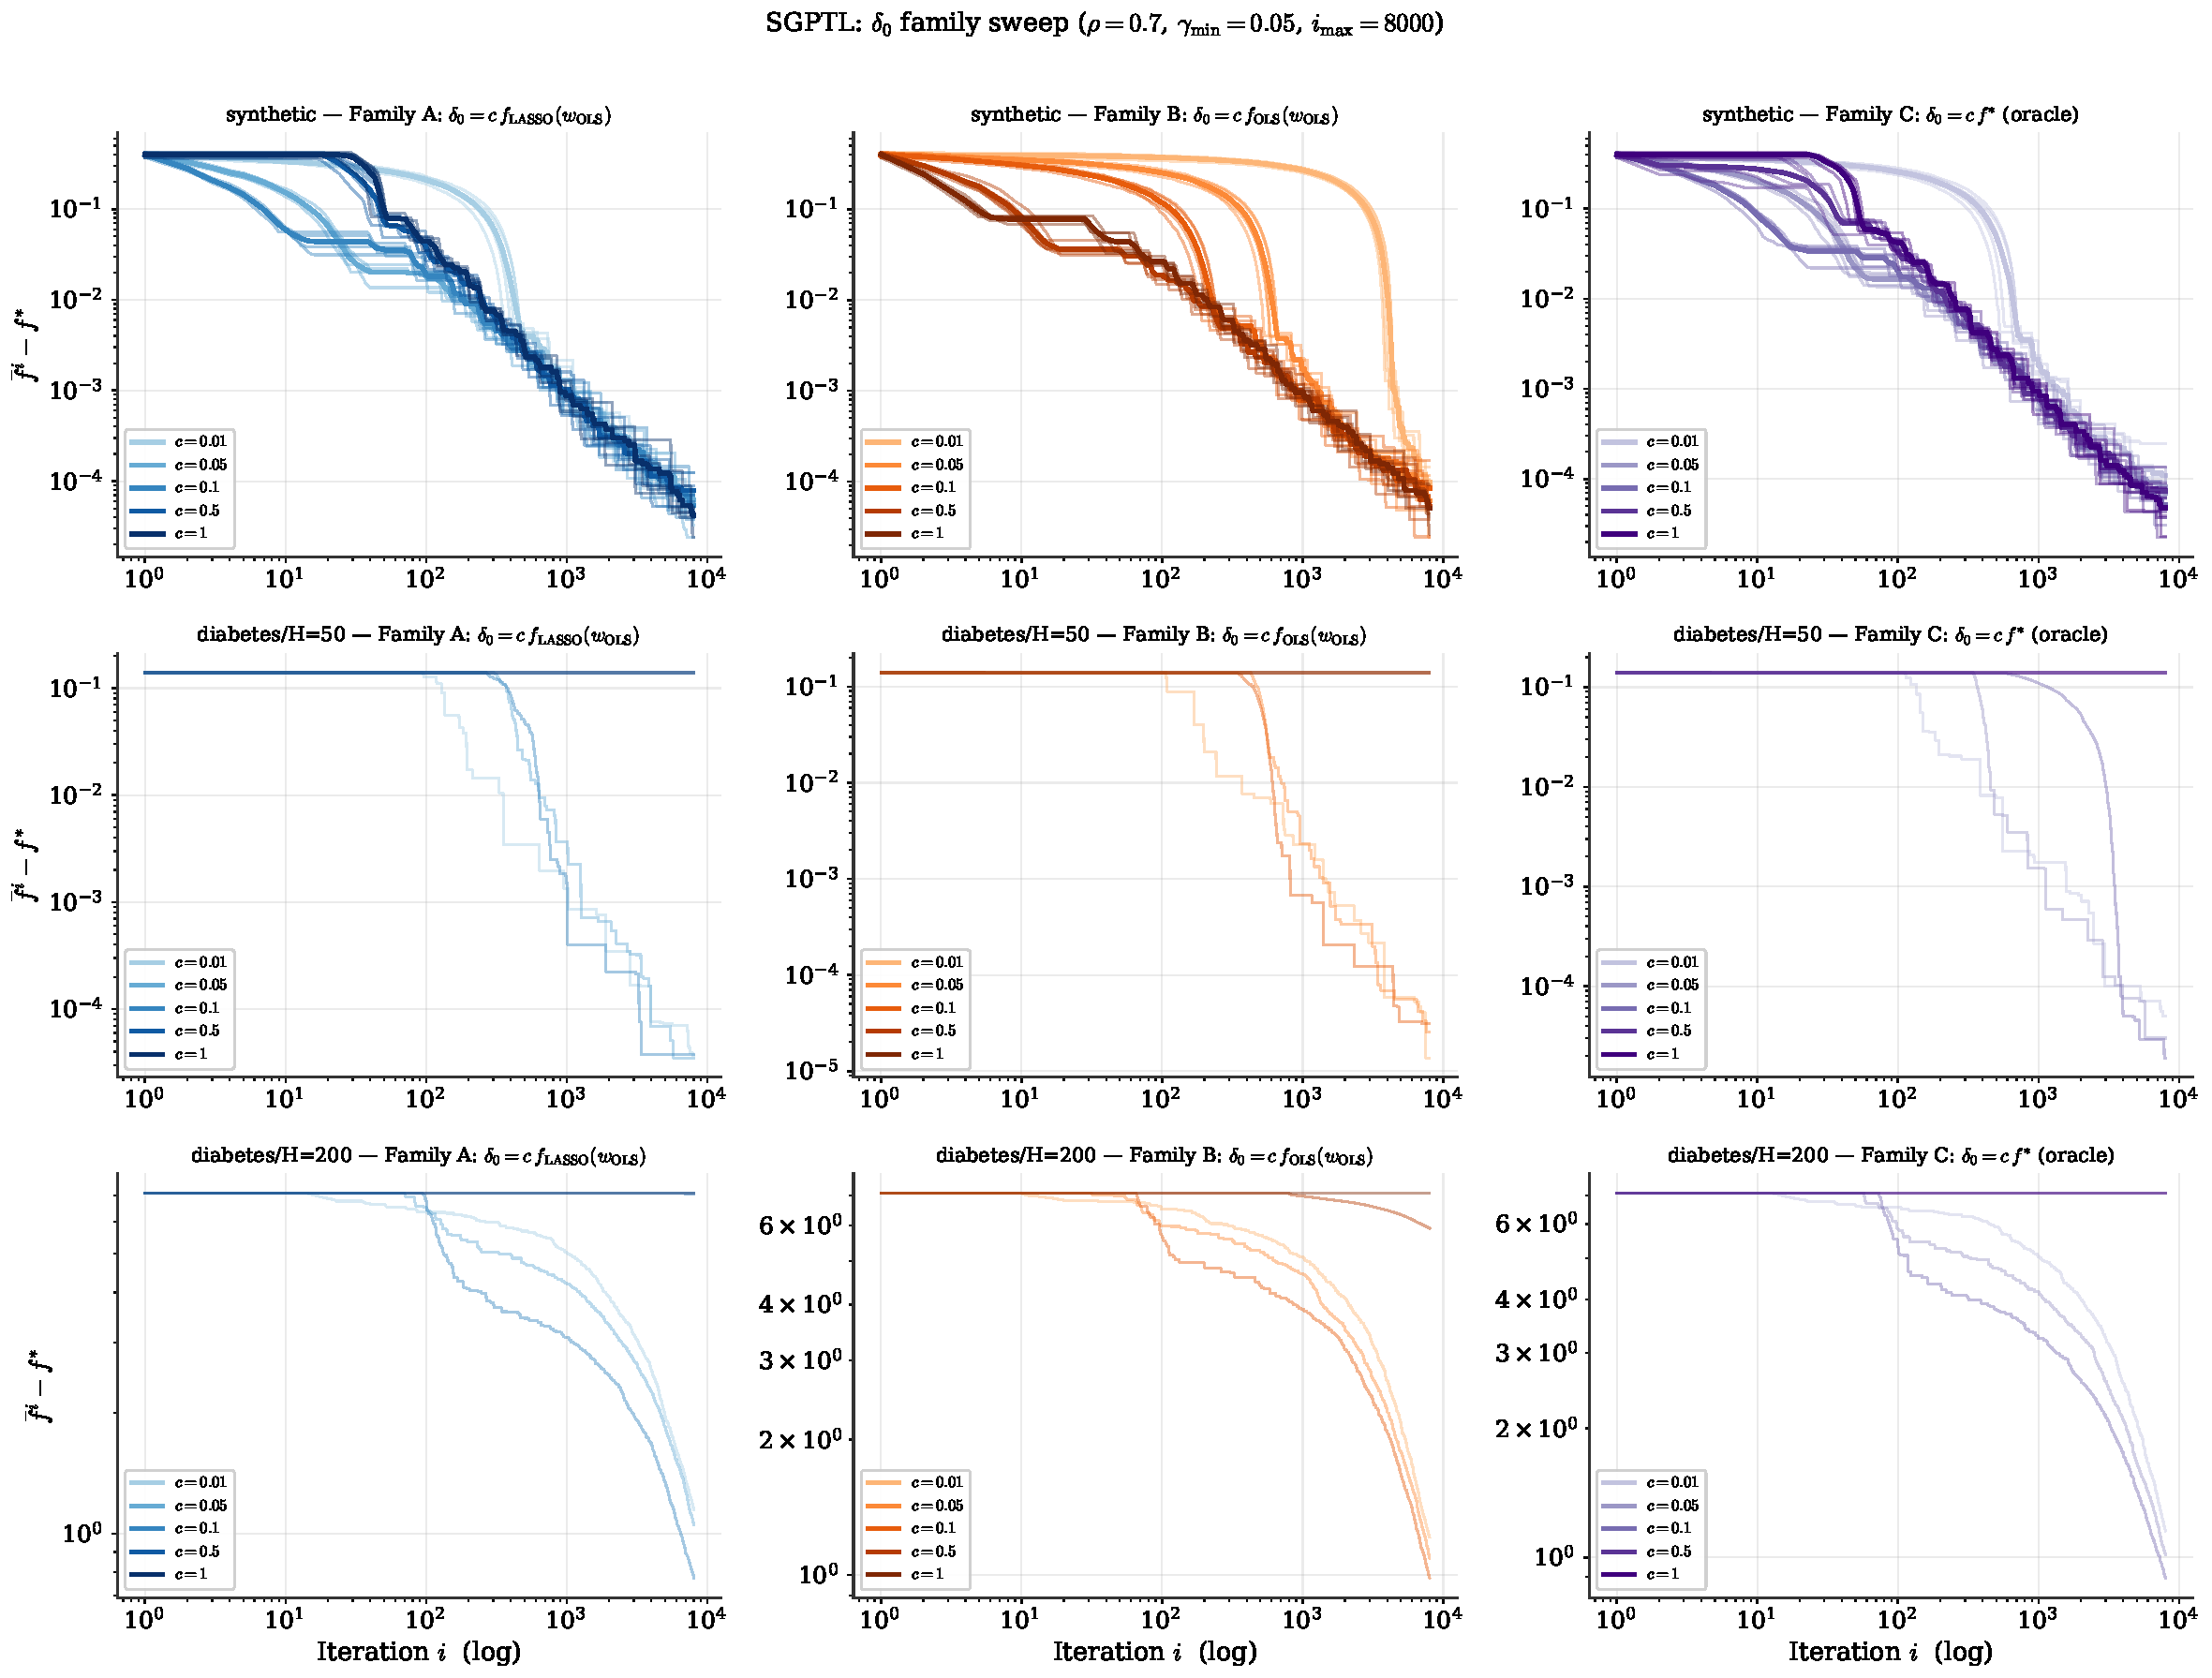
\includegraphics[width=\textwidth]{images/delta0_families.pdf}
    \caption{Sensitivity of the final record gap to $\delta_{0}$, three
    families across five instances (rows): synthetic ($5$ seeds, per-seed
    thin traces and aggregate-mean thick), \texttt{diabetes}~$H=50$
    (warm), \texttt{diabetes}~$H=200$ (warm), \texttt{california}~$H=50$
    (cold), \texttt{california}~$H=200$ (cold). All runs use
    $\lambda_\text{LASSO}=0.1$, $\rho=0.7$, $\gamma_{\min}=0.05$,
    $i_{\max}=8000$. Family~A: $\delta_{0}=c\,f(\mathbf{w}_{0})$
    (default). Family~B:
    $\delta_{0}=c\,\tfrac12\norm{\mathbf{X}\mathbf{w}_{0}-\mathbf{y}}^{2}$.
    Family~C: $\delta_{0}=c\,f^{*}$ (oracle, inadmissible). The
    Family~A/Family~C ratio falls in $[0.5,2.0]$ in every regime where
    SGPTL admits progress.}
    \label{fig:delta0-families}
\end{figure}

\chapter{IRLS warm vs cold start on the synthetic instance}
\label{app:irls-synth-warm-cold}

Section~\ref{sec:warm_cold} reports the warm-vs-cold contrast for IRLS on
the two real-data instances directly in the body
(Figure~\ref{fig:irls-warm-cold}). The analogue on the synthetic
benchmark ($H=100$, $M=300$, $\lambda_\text{LASSO}=0.1$, $200$ iterations,
$\varepsilon_\text{thr}=10^{-8}$) is reported here for completeness.

\begin{figure}[H]
    \centering
    
\includegraphics[width=0.8\textwidth]{images/irls_synthetic_warm_vs_cold.pdf}
    \caption{IRLS warm (OLS) vs cold ($\mathbf{w}_{0}=\mathbf{0}$) start
    on the synthetic instance ($H=100$, $M=300$,
    $\lambda_\text{LASSO}=0.1$, $k_{\max}=2000$,
    $\varepsilon_\text{thr}=10^{-8}$), log--log axes. Both starts converge
    to the $\varepsilon_\text{thr}$ floor ($\bar f - f^{*}\approx 1.8\cdot
    10^{-8}$) at iteration $940$ (warm) and $922$ (cold); the warm curve
    sits below the cold one throughout the descent, consistent with the
    multiplicative role of $\norm{\mathbf{w}_{0}-\mathbf{w}^{*}}$ in the
    bound of Theorem~\ref{thm:irls_convergence}.}
    \label{fig:irls-synth-warm-cold}
\end{figure}

\chapter{Derivation of the per-step Polyak inequality \texorpdfstring{\eqref{eq:def-step-polyak}}{}}
\label{app:def-step-polyak}

We derive the per-step descent estimate~\eqref{eq:def-step-polyak} of the proof of Theorem~\ref{thm:dsm_convergence} from three ingredients of~\cite{dantonio2009deflected}: the basic identity (2.9), Corollary~3.2, and the Polyak stepsize~\eqref{eq:sr_step}. The notation map between the paper and the report is $\alpha_k^{\text{paper}} \leftrightarrow \gamma_i$, $\beta_k^{\text{paper}} \leftrightarrow \beta_i$, $\nu_k^{\text{paper}} \leftrightarrow \alpha_i$; the exact-oracle regime fixes $\sigma_k = 0$, the uncorrected Polyak variant fixes the inner correction $\gamma_k$ of (3.1) of~\cite{dantonio2009deflected} to zero, and we evaluate the result at $\bar x = \mathbf{w}^*$.

\paragraph{Step 1 --- Identity (2.9).}
In the unconstrained case $X = \R^{H}$ no projection is needed and (2.9) of~\cite{dantonio2009deflected} reduces to expanding the square $\norm{\mathbf{w}_i - \alpha_i \mathbf{d}_i - \mathbf{w}^*}_{2}^{2}$:
\begin{equation}\label{eq:app-prf-29}
\norm{\mathbf{w}_{i+1} - \mathbf{w}^*}_{2}^{2} \;=\; \norm{\mathbf{w}_i - \mathbf{w}^*}_{2}^{2} \;-\; 2\alpha_i\,\langle \mathbf{d}_i, \mathbf{w}_i - \mathbf{w}^* \rangle \;+\; \alpha_i^{2}\,\norm{\mathbf{d}_i}_{2}^{2}.
\end{equation}

\paragraph{Step 2 --- Corollary~3.2 of~\cite{dantonio2009deflected}.}
Hypothesis~(2.13) is verified in step~(a) of the proof of Theorem~\ref{thm:dsm_convergence}, so Corollary~3.2 of~\cite{dantonio2009deflected} (specialised at $\bar x = \mathbf{w}^*$, $\sigma_k = 0$, $\bar\sigma_k = 0$) gives
\[
\langle \mathbf{d}_i,\, \mathbf{w}^* - \mathbf{w}_i \rangle \;\le\; \gamma_i\bigl(f^* - f(\mathbf{w}_i)\bigr) \;+\; \bigl[f(\mathbf{w}^*) - f^* + 0\bigr] \;=\; -\gamma_i\bigl(f(\mathbf{w}_i) - f^*\bigr),
\]
that is,
\begin{equation}\label{eq:app-prf-32}
\langle \mathbf{d}_i,\, \mathbf{w}_i - \mathbf{w}^* \rangle \;\ge\; \gamma_i\,\bigl(f(\mathbf{w}_i) - f^*\bigr).
\end{equation}
The factor $\gamma_i$ on the right-hand side (and not the full $1$ that convexity would give for the plain subgradient $\mathbf{g}_i$) is the deflection-induced loss: $\mathbf{d}_i$ is a convex combination involving past subgradients (those at $\mathbf{w}_{i-1}, \mathbf{w}_{i-2}, \dots$), so only the weight $\gamma_i$ on the current $\mathbf{g}_i$ can be certified to separate $\mathbf{w}_i$ from $\mathbf{w}^*$ by the subgradient inequality.

\paragraph{Step 3 --- Polyak stepsize substitution.}
We work in the regime where Lemma~3.8 of~\cite{dantonio2009deflected} has driven the target $f^{k}_{\mathrm{ref}} - \delta_{k}$ to $f^*$, so~\eqref{eq:sr_step} reads $\alpha_i = \beta_i (f(\mathbf{w}_i) - f^*)/\norm{\mathbf{d}_i}_{2}^{2}$. Substituting into the two non-constant terms of~\eqref{eq:app-prf-29} and applying~\eqref{eq:app-prf-32}:
\begin{align}
-2\alpha_i\,\langle \mathbf{d}_i, \mathbf{w}_i - \mathbf{w}^* \rangle
\;&\overset{\eqref{eq:app-prf-32}}{\le}\; -2\alpha_i\,\gamma_i\bigl(f(\mathbf{w}_i) - f^*\bigr)
\;=\; -2\,\beta_i\,\gamma_i\,\frac{(f(\mathbf{w}_i) - f^*)^{2}}{\norm{\mathbf{d}_i}_{2}^{2}}, \label{eq:app-prf-step3a}\\
\alpha_i^{2}\,\norm{\mathbf{d}_i}_{2}^{2}
\;&=\; \biggl(\frac{\beta_i\,(f(\mathbf{w}_i) - f^*)}{\norm{\mathbf{d}_i}_{2}^{2}}\biggr)^{2}\,\norm{\mathbf{d}_i}_{2}^{2}
\;=\; \beta_i^{2}\,\frac{(f(\mathbf{w}_i) - f^*)^{2}}{\norm{\mathbf{d}_i}_{2}^{2}}. \label{eq:app-prf-step3b}
\end{align}

\paragraph{Step 4 --- Collecting.}
Summing~\eqref{eq:app-prf-step3a} and~\eqref{eq:app-prf-step3b} into~\eqref{eq:app-prf-29},
\[
\norm{\mathbf{w}_{i+1} - \mathbf{w}^*}_{2}^{2}
\;\le\; \norm{\mathbf{w}_i - \mathbf{w}^*}_{2}^{2}
\;-\; \bigl(2\,\beta_i\,\gamma_i \;-\; \beta_i^{2}\bigr)\,\frac{(f(\mathbf{w}_i) - f^*)^{2}}{\norm{\mathbf{d}_i}_{2}^{2}},
\]
and factoring $\beta_i$,
\[
\norm{\mathbf{w}_{i+1} - \mathbf{w}^*}_{2}^{2}
\;\le\; \norm{\mathbf{w}_i - \mathbf{w}^*}_{2}^{2}
\;-\; \beta_i\,(2\gamma_i - \beta_i)\,\frac{(f(\mathbf{w}_i) - f^*)^{2}}{\norm{\mathbf{d}_i}_{2}^{2}},
\]
which is~\eqref{eq:def-step-polyak}. This matches eq.~(3.17) of~\cite{dantonio2009deflected} under the notation map above.

\paragraph{Specialisation to Algorithm~\ref{alg:dsm}.}
Algorithm~\ref{alg:dsm} sets $\beta_i = \min(1, \gamma_i) = \gamma_i$ (because the clip~\eqref{eq:gamma_star} keeps $\gamma_i \le 1$ at every iteration), so the descent factor collapses to
\[
\beta_i\,(2\gamma_i - \beta_i) \;=\; \gamma_i\,(2\gamma_i - \gamma_i) \;=\; \gamma_i^{2} \;\ge\; \gamma_{\min}^{2},
\]
which is the form fed back into the telescoping argument of the proof of Theorem~\ref{thm:dsm_convergence}.

\chapter{Derivation of the optimal deflection \texorpdfstring{$\gamma^{*}$}{gamma*}}
\label{app:gamma-star}

We derive the closed form~\eqref{eq:gamma_star} for the minimiser of
\[
h(\gamma) \;:=\; \norm{\gamma\,\mathbf{g}_i + (1-\gamma)\,\mathbf{d}_{i-1}}_2^{2}
\]
on $\R$, then justify the clip to $[\gamma_{\min}, 1]$. Expanding by bilinearity of the inner product,
\[
h(\gamma) \;=\; \gamma^{2}\,\norm{\mathbf{g}_i}_2^{2} \;+\; 2\,\gamma(1-\gamma)\,\inner{\mathbf{g}_i}{\mathbf{d}_{i-1}} \;+\; (1-\gamma)^{2}\,\norm{\mathbf{d}_{i-1}}_2^{2}.
\]
Collecting powers of $\gamma$,
\begin{equation}\label{eq:app-gamma-parabola}
h(\gamma) \;=\; \underbrace{\bigl(\norm{\mathbf{g}_i}_2^{2} - 2\inner{\mathbf{g}_i}{\mathbf{d}_{i-1}} + \norm{\mathbf{d}_{i-1}}_2^{2}\bigr)}_{=\,\norm{\mathbf{g}_i - \mathbf{d}_{i-1}}_2^{2}}\,\gamma^{2} \;+\; 2\,\bigl(\inner{\mathbf{g}_i}{\mathbf{d}_{i-1}} - \norm{\mathbf{d}_{i-1}}_2^{2}\bigr)\,\gamma \;+\; \norm{\mathbf{d}_{i-1}}_2^{2},
\end{equation}
a parabola in $\gamma$ with leading coefficient $\norm{\mathbf{g}_i - \mathbf{d}_{i-1}}_2^{2} \ge 0$.

\paragraph{Degenerate case $\mathbf{g}_i = \mathbf{d}_{i-1}$.}
The leading coefficient vanishes and $h(\gamma) \equiv \norm{\mathbf{d}_{i-1}}_2^{2}$ is constant on $\R$; moreover the deflected direction $\mathbf{d}_i = \gamma\,\mathbf{g}_i + (1-\gamma)\,\mathbf{d}_{i-1} = \mathbf{d}_{i-1}$ for every $\gamma$, so the algorithm is insensitive to the choice. We set $\gamma_i = 1$ by convention (consistent with the unclipped Polyak first step $\mathbf{d}_0 = \mathbf{g}_0$).

\paragraph{Generic case $\mathbf{g}_i \neq \mathbf{d}_{i-1}$.}
The leading coefficient is strictly positive, so $h$ is strictly convex with a unique unconstrained minimiser. Setting $h^{\prime}(\gamma) = 0$ in~\eqref{eq:app-gamma-parabola},
\[
2\,\norm{\mathbf{g}_i - \mathbf{d}_{i-1}}_2^{2}\,\gamma \;+\; 2\,\bigl(\inner{\mathbf{g}_i}{\mathbf{d}_{i-1}} - \norm{\mathbf{d}_{i-1}}_2^{2}\bigr) \;=\; 0 \quad\Longrightarrow\quad \gamma^{*} \;=\; \frac{\norm{\mathbf{d}_{i-1}}_2^{2} - \inner{\mathbf{g}_i}{\mathbf{d}_{i-1}}}{\norm{\mathbf{g}_i - \mathbf{d}_{i-1}}_2^{2}},
\]
which is~\eqref{eq:gamma_star}.

\paragraph{Projection onto $[\gamma_{\min}, 1]$.}
Since the parabola opens upward, $h$ is decreasing on $(-\infty, \gamma^{*}]$ and increasing on $[\gamma^{*}, +\infty)$. The constrained minimum over $[\gamma_{\min}, 1]$ is therefore
\[
\gamma_i \;=\; \begin{cases}
\gamma_{\min} & \text{if } \gamma^{*} < \gamma_{\min}, \\
\gamma^{*} & \text{if } \gamma^{*} \in [\gamma_{\min}, 1], \\
1 & \text{if } \gamma^{*} > 1,
\end{cases}
\qquad\text{i.e.\ } \gamma_i \;=\; \min\bigl(1,\; \max(\gamma_{\min},\, \gamma^{*})\bigr).
\]
The two clip endpoints serve different purposes: the lower clip $\gamma_{\min}$ enforces the uniform bound $\beta^{*} > 0$ of condition~(3.5) of~\cite{dantonio2009deflected} (Section~\ref{sec:dsm_convergence_conditions}); the upper clip at $1$ keeps $\gamma_i \in (0,1]$ so that $\mathbf{d}_i$ is a convex combination of $\mathbf{g}_i$ and $\mathbf{d}_{i-1}$, a property used in the per-step descent estimate of Appendix~\ref{app:def-step-polyak}.

\paragraph{Interpretation.}
The denominator $\norm{\mathbf{g}_i - \mathbf{d}_{i-1}}_2^{2}$ measures how far the current subgradient is from the previous deflected direction: large values shrink $\gamma^{*}$ and tilt the deflected direction toward memory $\mathbf{d}_{i-1}$. The numerator $\norm{\mathbf{d}_{i-1}}_2^{2} - \inner{\mathbf{g}_i}{\mathbf{d}_{i-1}}$ captures alignment: it is small (so $\gamma^{*}$ is small) when $\mathbf{g}_i$ and $\mathbf{d}_{i-1}$ point in similar directions, and large when they oppose each other.

In the zig-zag regime $\mathbf{g}_i \approx -\mathbf{d}_{i-1}$ with $\norm{\mathbf{g}_i}_2 \approx \norm{\mathbf{d}_{i-1}}_2$, the numerator is approximately $\norm{\mathbf{d}_{i-1}}_2^{2} + \norm{\mathbf{d}_{i-1}}_2^{2} = 2\,\norm{\mathbf{d}_{i-1}}_2^{2}$ while the denominator is approximately $\norm{2\,\mathbf{d}_{i-1}}_2^{2} = 4\,\norm{\mathbf{d}_{i-1}}_2^{2}$, so $\gamma^{*} \approx 1/2$: the deflected direction $\mathbf{d}_i$ splits evenly between $\mathbf{g}_i$ and $\mathbf{d}_{i-1}$ and the oscillatory component cancels.
